\section{Methodology}
\label{sec:methodology}

\begin{figure*}[t]
    \centering
    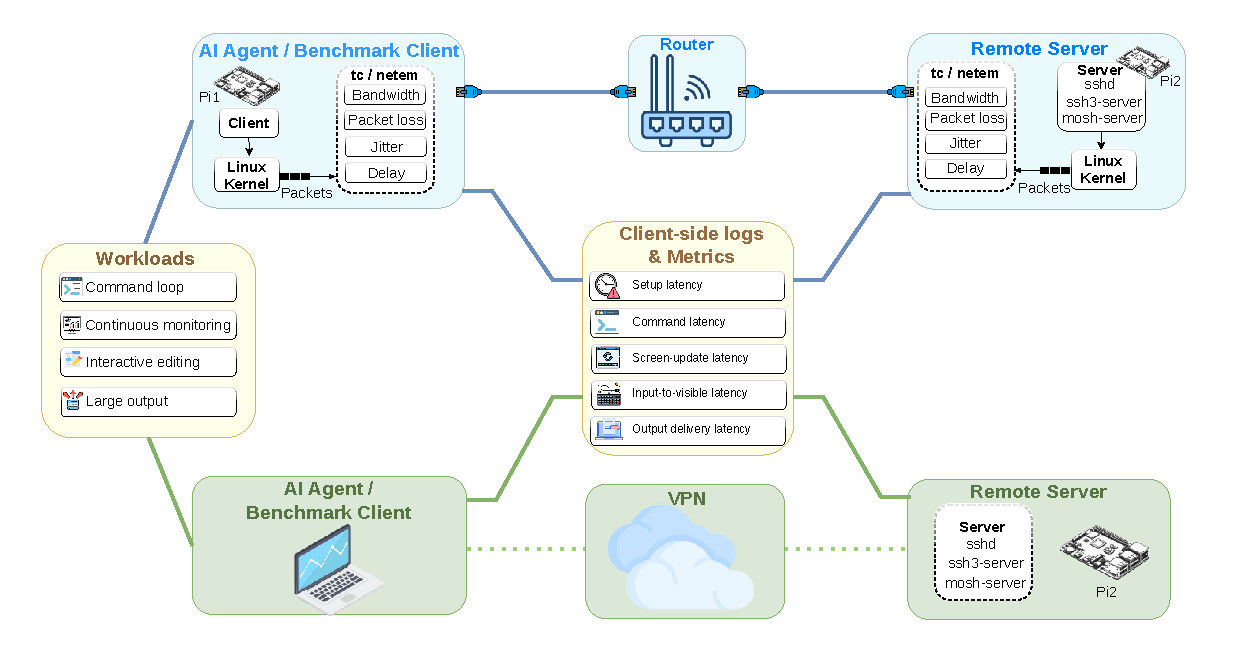
\includegraphics[width=\textwidth]{figs/measurement_framework.pdf}
    \caption{Measurement framework for SSHv2, Mosh, and SSH3 under interactive AI agent workloads.}
    \label{fig:measurement-framework}
\end{figure*}

This section presents the experimental methodology used to evaluate SSHv2, Mosh, and SSH3 under interactive AI agent terminal workloads. We quantify protocol behavior using terminal events observable at the benchmark client rather than relying only on network-level indicators such as round-trip time or throughput.

\subsection{Measurement Framework}
\label{subsec:measurement-framework}

Figure~\ref{fig:measurement-framework} illustrates the measurement framework. The benchmark client establishes remote sessions, generates workloads, sends commands or probe characters, observes terminal output, and records timestamps for each measurement event. The same workload suite is executed over SSHv2, Mosh, and SSH3. Traffic then traverses either a controlled LAN environment with tc/netem-based emulation or a VPN-based environment.

On the remote server, sshd, mosh-server, and ssh3-server are installed and listen concurrently. However, only one protocol is active in each experimental run. This design avoids cross-protocol interference during measurement while keeping the server hardware, operating system, account configuration, and workload content consistent across protocols. The controlled LAN environment isolates the effect of configured network impairments, whereas the VPN-based environment captures behavior over a practical overlay deployment path.

\subsection{Experimental Setup and Protocol Implementations}
\label{subsec:protocol-implementations-measurement-semantics}

In the controlled environment, two Raspberry Pi 4 devices serve as the benchmark client (Pi1) and the remote server (Pi2), connected directly via Ethernet (eth0). Network impairments are applied using Linux tc/netem. In the VPN-based environment, the benchmark client runs on an Acer Nitro AN515-58 laptop running Linux 6.19.11-1-cachyos, which connects through a VPN tunnel to the same remote server (Pi2).

The benchmark client runs Python scripts based on pexpect to establish sessions, issue commands or probes, observe terminal output, and write CSV logs. Each measurement record is associated with protocol, scenario, workload, command or probe type, session ID, sample ID, timestamp information, and success or failure status.

The controlled environment uses three impairment profiles, shown in Table~\ref{tab:network-scenarios}: Low, Medium, and High. These labels indicate increasing network degradation rather than absolute worst-case Internet conditions. Low represents a stable LAN-like setting, Medium introduces noticeable delay, jitter, and packet loss, and High stresses the protocols with lower bandwidth, higher delay, and higher loss.

Because Linux netem applies impairments only to the egress direction, the same configuration is applied on both the client and the server to emulate bidirectional degradation. Thus, when the configured one-way delay is $D$ ms per side, the expected round-trip time is approximately $2D$ ms, excluding jitter and host-processing overhead. The loss values in Table~\ref{tab:network-scenarios} are also per-egress values. If packet loss $p$ is applied in both directions, the approximate bidirectional loss exposure for a request-response exchange is $1-(1-p)^2$.

\begin{table}[t]
\centering
\caption{Per-egress network scenarios used in the controlled environment and VPN environment.}
\label{tab:network-scenarios}
\begin{tabular}{lcccc}
\toprule
Scenario & Bandwidth & OWD & Jitter & Loss/egress \\
\midrule
Low & 100 Mbps & 10 ms & 0 ms & 0\% \\
Medium & 40 Mbps & 50 ms & 4 ms & 1.5\% \\
High & 10 Mbps & 100 ms & 16 ms & 3\% \\
VPN & N/A & N/A & N/A & N/A \\
\bottomrule
\end{tabular}
\end{table}

We evaluate concrete protocol implementations rather than abstract protocol models. SSHv2 is implemented with OpenSSH 9.2p1 and OpenSSL 3.0.17. Mosh is implemented with Mosh 1.4.0 and uses the standard SSH bootstrap procedure before switching to its interactive UDP channel. SSH3 is implemented using francoismichel/ssh3 version 0.1.7 and connects to the /ssh3-term server endpoint.

All protocols use the same remote account, SSH key material, server host, terminal environment, and workload content. SSHv2 is invoked through OpenSSH with pseudo-terminal allocation enabled. Mosh is invoked through the Mosh client using the same SSH bootstrap command, with local input prediction consistently enabled across Mosh trials. SSH3 is invoked through the SSH3 client with the corresponding private key and endpoint configuration. Runtime options, including source IP, identity file, host-key policy, SSH3 mode, and Mosh prediction mode, are recorded in the experiment metadata or run scripts.

Because the evaluated protocols do not expose identical terminal semantics, all metrics are defined using events observable at the benchmark client, including prompt arrival, completion-marker visibility, and character visibility. The interpretation of Mosh measurements follows the protocol-level trade-off discussed in Section~\ref{subsec:protocols}: input latency reflects visible terminal responsiveness, while large-output latency reflects observable terminal completion rather than byte-complete delivery.

\subsection{Application Workloads}
\label{subsec:application-workloads}

The benchmark includes three workloads: command loop (W1), large-output commands (W2), and interactive editing (W3, with single-pane and 5-pane variants). These workloads represent common interaction patterns of interactive AI agents operating through a remote terminal: issuing short commands, receiving large outputs, and performing interactive editing while one or multiple terminal panes remain active. The benchmark mechanism follows the client-side observation path in Figure~\ref{fig:measurement-framework}: prompt markers, completion markers, or client-side echo observations are used to identify the start and end of each measurement.

\paragraph{Command loop (W1).}
The command-loop workload consists of four short commands that produce small output ($\leq$1\,KB): \texttt{ls}, \texttt{df~-h}, \texttt{grep~-n~root~/etc/passwd}, and \texttt{git~status}. This workload captures short request-response interactions in which an agent issues a command, waits for the resulting output, and uses the observation to determine the next action.

\paragraph{Large-output commands (W2).}
The large-output workload consists of \texttt{find~/}, \texttt{ps~aux}, and \texttt{docker~logs}, with a 20\,s per-sample timeout. These commands produce tens of kilobytes of output and capture cases in which the agent must wait for a large terminal output to reach an observable completion state before continuing.

\paragraph{Basic interactive editing (W3, single-pane).}
The basic interactive-editing workload evaluates input visibility in \textit{interactive shell}, \textit{vim}, and \textit{nano}. It captures the latency between sending an input character and observing that character at the client side.

\paragraph{5-pane interactive editing (W3, multi-pane).}
The 5-pane interactive-editing workload uses a tmux session to emulate editing under concurrent terminal activity. Pane 0 receives the probe stream, while panes 1-4 continuously generate background output and redraw load. This setting represents a terminal session in which the agent edits or types in one pane while other panes concurrently update monitoring output, logs, or command results.

For each protocol, workload, and command or probe combination, the experiment opens 10 independent sessions, and each session collects 100 measured samples unless otherwise noted in the dataset metadata. Within each scenario, combinations of protocol, workload, and command or probe type are shuffled using a fixed seed before execution. This reduces order effects caused by cache state, device temperature, run order, or background variation. The seed and shuffle state are stored with the metadata so that the experiment order can be reconstructed.

\subsection{Measurement Metrics}
\label{subsec:measurement-metrics}

All local timestamps are recorded with nanosecond resolution and converted to milliseconds during preprocessing. Since all latency metrics share the same event-difference structure, we define a general latency metric as
\begin{equation}
L_m = t_{\mathrm{obs}}^{m} - t_{\mathrm{init}}^{m},
\end{equation}
where $m$ identifies the measurement type, $t_{\mathrm{init}}^{m}$ is the 
client-side timestamp when the action is initiated, and $t_{\mathrm{obs}}^{m}$ is the client-side timestamp when the corresponding terminal event becomes visible. The two timestamps are instantiated as follows.

\paragraph{Session setup ($L_{\mathrm{setup}}$)}
From the client launching the protocol command to the first remote shell prompt becoming visible. Captures the delay before the agent can issue commands in a newly established session.

\paragraph{Command completion ($L_{\mathrm{cmd}}$)}
From sending a short command to observing the completion marker. Captures short request-response interactions in agent command loops.

\paragraph{Output completion ($L_{\mathrm{out}}$)}
From sending a large-output command to the completion marker becoming visible. For Mosh, this reflects observable terminal completion rather than byte-complete delivery (Section~\ref{subsec:protocol-implementations-measurement-semantics}).

\paragraph{Input-to-visible ($L_{\mathrm{input}}$)}
From sending a probe character to the character becoming visible. Measured in \textit{interactive shell}, \textit{vim}, and \textit{nano} contexts.

\paragraph{5-pane input-to-visible ($L_{\mathrm{input}}^{\mathrm{5pane}}$)}
Same definition as $L_{\mathrm{input}}$, applied to pane 0 of a tmux session while anes 1-4 generate background output and redraw load.

\subsection{Data Collection and Statistical Analysis}
\label{subsec:data-collection-statistical-analysis}

All measurement records are stored at the sample level. Each record includes the protocol, scenario, workload, command or probe type, session ID, sample ID, measured latency, success or failure status, and error information when applicable. Failures, timeouts, and samples that do not match the expected marker are logged separately rather than discarded, allowing the analysis to capture both latency and protocol robustness.

For each protocol, scenario, and workload combination, we report the number of valid samples $N$, failures, success rate, and latency statistics. The summary includes mean, median, standard deviation, the 95\% confidence interval of the mean, minimum, maximum, 95th percentile, and 99th percentile. The median represents typical behavior, while the 95th and 99th percentiles capture tail latency that an interactive AI agent may experience during long terminal interaction loops.